\documentclass[conference]{IEEEtran}
\IEEEoverridecommandlockouts

\usepackage{cite}
\usepackage{amsmath,amssymb,amsfonts}
\usepackage{algorithmic}
\usepackage{graphicx}
\usepackage{textcomp}
\usepackage{hyperref}
\usepackage{xcolor}
\def\BibTeX{{\rm B\kern-.05em{\sc i\kern-.025em b}\kern-.08em
    T\kern-.1667em\lower.7ex\hbox{E}\kern-.125emX}}
\begin{document}

\title{Optical Character Recognition from Images Using a CNN–Transformer Architecture in PyTorch}

\author{\IEEEauthorblockN{1\textsuperscript{st} Veljko Petkovic}
\IEEEauthorblockA{\textit{Faculty of Sciences and Mathematics} \\
\textit{University of Nis}\\
Nis, Serbia \\
veljko.petko0022@gmail.com}
}

\maketitle

\begin{abstract}

This paper presents the development of a deep learning–based system for automatic recognition of alphanumeric characters from images. This approach relies on a convolutional neural network for visual feature extraction combined with sequence modeling and the Connectionist Temporal Classification (CTC) loss, enabling end-to-end optical character recognition without explicit character segmentation. A key contribution of this work is the use of synthetically generated training data, which allows precise control over text length, character distribution, and image properties. The entire system is implemented in the PyTorch framework. Experimental results demonstrate that the proposed model achieves high recognition accuracy and exhibits strong generalization capabilities on previously unseen samples.

\end{abstract}

\begin{IEEEkeywords}
Optical Character Recognition, CNN, Transformer, CTC Loss, Sequence Modeling
\end{IEEEkeywords}

\section{\textbf{Introduction}}

Optical Character Recognition (OCR) is a fundamental problem in computer vision with widespread applications in document digitization, license plate recognition, automated form processing, and assistive technologies. Traditional OCR systems were primarily based on handcrafted features and rule-based pipelines, which limited their robustness when exposed to variations in font styles, image noise, distortions, and illumination conditions.

Recent advances in deep learning have significantly improved OCR performance by enabling models to learn discriminative features directly from raw image data. Convolutional Neural Networks (CNNs) have proven particularly effective for extracting spatial features, while recurrent and attention-based models allow sequence-level reasoning required for reading text. End-to-end OCR architectures eliminate the need for manual character segmentation, which is often error prone in real world scenarios.

This work focuses on alphanumeric character recognition from images, where the input may contain sequences of variable length composed of letters, digits, and whitespace. The goal is to design a robust OCR pipeline that combines synthetic data generation, convolutional feature extraction, and sequence modeling within a unified framework implemented in PyTorch.

\section{\textbf{Methodology}}

\subsection{Data Generation and Preparation}

The training dataset used in this project is generated synthetically to ensure full control over the content  of the data. Each image contains a randomly generated alphanumeric string with a length ranging from a minimum of 3 to a maximum of 14 characters. The character set includes uppercase and lowercase letters, digits, and spaces.

\begin{figure}[h]
    \centering
    
\includegraphics[width=0.25\textwidth]{000082.png}
    \caption{Generated image 000082.png using images\_generator.ipynb}
    \label{fig:image_example1}
\end{figure}

Synthetic image generation allows systematic variation of fonts (DejaVu sans, Arial and Liberation Sans), spacing, and text composition, reducing dependency on manually labeled real world datasets. Total of 50.000 images are rendered in grayscale with a fixed resolution of 280 × 70 pixels, ensuring a consistent input size for the neural network. Corresponding labels are stored in a CSV file, mapping each image filename to its text sequence.

During dataset preparation, textual labels are normalized by removing unsupported characters, collapsing multiple spaces, and enforcing length constraints. Each character is encoded using an integer based vocabulary, where index zero is reserved for the CTC blank symbol. The dataset is split into training, validation, and test subsets using an 80/10/10 ratio. Samples with missing images or invalid labels are discarded prior to splitting.

Input images are normalized to the range [0, 1] and resized when necessary. A custom collate function is used during data loading to handle variable length target sequences, concatenating label tensors and maintaining sequence length metadata required by the CTC loss.

\subsection{Model Architecture}

The OCR model follows a CNN-based sequence recognition architecture inspired by CRNN designs, enhanced with a Transformer encoder for improved modeling.

The network consists of multiple convolutional layers with increasing channel depth, combined with normalization and ReLU activation functions. Max-pooling operations are applied selectively to reduce the height of the feature maps while preserving the width dimension, which is interpreted as the temporal axis of the sequence. This design enables the model to convert a two-dimensional image into a one-dimensional sequence of feature vectors.

After convolutional processing, the height dimension is collapsed to a size of 1 using a convolutional layer with a kernel spanning the entire feature map height. The resulting tensor represents a sequence of feature embeddings related to horizontal positions in the input image.

To model long-range relationships between characters, the sequence is passed through a Transformer encoder composed of multiple self-attention layers. Sinusoidal positional encoding is added to preserve positional information within the sequence. The Transformer encoder improves reliability to character spacing variations and helps resolve confusions between visually similar characters.

The final classification layer is a fully connected linear projection that maps each sequence embedding to a probability distribution over all character classes plus the CTC blank symbol.

\begin{figure}[h]
    \centering
    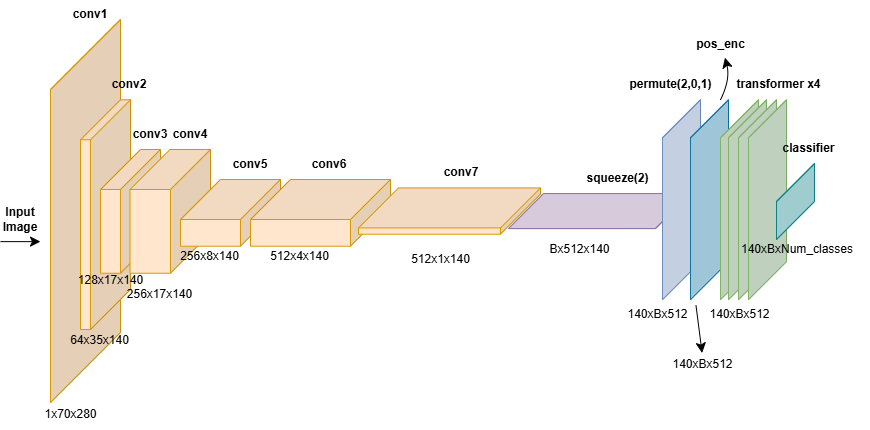
\includegraphics[width=0.5\textwidth]{model.png}
    \caption{Model architecture}
    \label{fig:image_example2}
\end{figure}

\subsection{Training Procedure}

The model is trained end-to-end using the CTC loss function, which aligns predicted character sequences with ground-truth labels without requiring explicit segmentation. The CTC loss enables flexible handling of variable-length outputs and repeated predictions.

Regularization techniques, including normalization layers and dropout, are applied to improve generalization. Due to the computational demands of convolutional and attention-based layers, training is performed using GPU acceleration. All experiments are conducted on Google Colaboratory using an NVIDIA L4 GPU.

Training is performed using the Adam optimizer with a learning rate schedule with a linear warm-up phase followed by cosine decay. Mini-batch gradient descent is used, with batch sizes selected based on available GPU memory. Model performance is monitored on a validation set to detect overfitting, and the best-performing model checkpoint is selected based on the validation loss.

\begin{figure}[h]
    \centering
    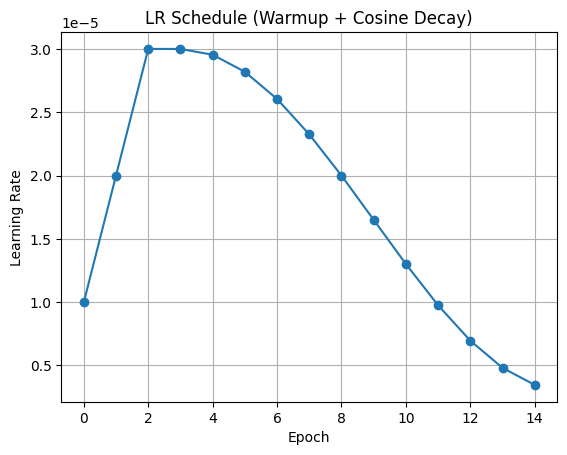
\includegraphics[width=0.4\textwidth]{lr.png}
    \caption{Learning rate progression during training}
    \label{fig:image_example3}
\end{figure}

The training process converges smoothly, with both training and validation losses decreasing consistently across epochs. The Character Error Rate (CER) on the validation set reaches its lowest value of 0.000523 at the final epoch, indicating good generalization without signs of overfitting. Evaluation on the test set results in a CER of 0.0005, which is consistent with the validation performance and shows that the model performs well on previously unseen data. The entire training process is completed in under 28 minutes.

\section{\textbf{Results}}

Experimental evaluation shows that the proposed model achieves high character-level and sequence-level accuracy on the validation dataset. The use of synthetic data enables the model to generalize well to unseen text combinations, even when character spacing and composition vary. Figure~\ref{fig:qualitative_results} presents qualitative examples comparing input images with the corresponding model predictions. These qualitative evaluations are generated using the inference pipeline implemented in the model\_testing.ipynb notebook.

\begin{figure}[h]
    \centering
    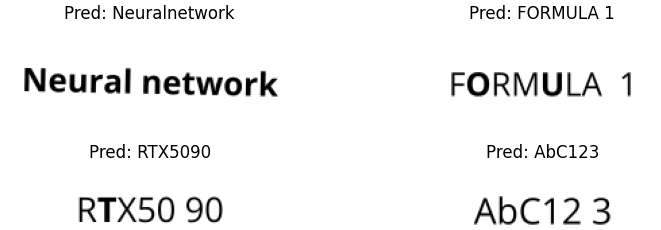
\includegraphics[width=0.4\textwidth]{preds.png}
    \caption{Qualitative results}
    \label{fig:qualitative_results}
\end{figure}

The qualitative examples further illustrate the behavior of the proposed model on individual samples. In the shown cases, the model correctly recognizes complete words such as “Neural network” and “FORMULA 1”, as well as alphanumeric strings including hardware identifiers. Minor errors can be observed in a small number of predictions, primarily related to character spacing or the separation of adjacent characters (missing or misplaced spaces). These errors are consistent with the character-level evaluation metrics and are limited, suggesting that the model maintains reliable performance across different text formats.

\section{\textbf{Conclusion}}

This work demonstrates that accurate alphanumeric OCR can be achieved using a CNN-based sequence recognition model implemented in PyTorch. By combining synthetic data generation, convolutional feature extraction, and Transformer-based sequence modeling with CTC loss, the proposed system performs robust end-to-end text recognition without manual segmentation.

The results confirm that synthetic datasets are a practical alternative to large annotated real-world datasets when carefully designed. Future improvements may include advanced data augmentation, integration of language models for post-processing, and deployment-oriented optimizations such as model quantization and pruning.


\begin{thebibliography}{00}
\bibitem{b1} Graves, A., Fernández, S., Gomez, F., \& Schmidhuber, J. Connectionist Temporal Classification: Labelling Unsegmented Sequence Data with Recurrent Neural Networks. IEEE, 2006.

\bibitem{b2} Shi, B., Bai, X., \& Yao, C. An End-to-End Trainable Neural Network for Image-Based Sequence Recognition and Its Application to Scene Text Recognition. IEEE TPAMI, 2017.

\bibitem{b3} Vaswani, A. et al. Attention Is All You Need. NeurIPS, 2017.

\bibitem{b4} Goodfellow, I., Bengio, Y., \& Courville, A. Deep Learning. MIT Press, 2016.

\end{thebibliography}
\end{document}
